\documentclass[sigchi]{acmart}

\usepackage{booktabs} % For formal tables

% Copyright
%\setcopyright{none}
%\setcopyright{acmcopyright}
%\setcopyright{acmlicensed}
%\setcopyright{rightsretained}
%\setcopyright{usgov}
%\setcopyright{usgovmixed}
%\setcopyright{cagov}
\setcopyright{licensedcagov}
%\setcopyright{cagovmixed}
%\setcopyright{licensedothergov}

% DOI
\acmDOI{10.475/123_4}

% ISBN
\acmISBN{123-4567-24-567/08/06}

%Conference
\acmConference[WOODSTOCK'97]{ACM Woodstock conference}{July 1997}{El
  Paso, Texas USA}
\acmYear{1997}
\copyrightyear{2016}

\acmPrice{15.00}


\begin{document}
\title{This is the Greatest and Best Paper in the World (Tribute)}
\titlenote{Produces the permission block, and
  copyright information}
\subtitle{Extended Abstract}
\subtitlenote{The full version of the author's guide is available as
  \texttt{acmart.pdf} document}

\author{Ben Trovato}
\authornote{Dr.~Trovato insisted his name be first.}
\orcid{1234-5678-9012}
\affiliation{%
  \institution{Institute for Clarity in Documentation}
  \streetaddress{P.O. Box 1212}
  \city{Dublin}
  \state{Ohio}
  \postcode{43017-6221}
}
\email{trovato@corporation.com}

\author{G.K.M. Tobin}
\authornote{The secretary disavows any knowledge of this author's actions.}
\affiliation{%
  \institution{Institute for Clarity in Documentation}
  \streetaddress{P.O. Box 1212}
  \city{Dublin}
  \state{Ohio}
  \postcode{43017-6221}
}
\email{webmaster@marysville-ohio.com}

\author{Lars Th{\o}rv{\"a}ld}
\authornote{This author is the
  one who did all the really hard work.}
\affiliation{%
  \institution{The Th{\o}rv{\"a}ld Group}
  \streetaddress{1 Th{\o}rv{\"a}ld Circle}
  \city{Hekla}
  \country{Iceland}}
\email{larst@affiliation.org}

\author{Valerie B\'eranger}
\affiliation{%
  \institution{Inria Paris-Rocquencourt}
  \city{Rocquencourt}
  \country{France}
}
\author{Aparna Patel}
\affiliation{%
 \institution{Rajiv Gandhi University}
 \streetaddress{Rono-Hills}
 \city{Doimukh}
 \state{Arunachal Pradesh}
 \country{India}}
\author{Huifen Chan}
\affiliation{%
  \institution{Tsinghua University}
  \streetaddress{30 Shuangqing Rd}
  \city{Haidian Qu}
  \state{Beijing Shi}
  \country{China}}

\author{Charles Palmer}
\affiliation{%
  \institution{Palmer Research Laboratories}
  \streetaddress{8600 Datapoint Drive}
  \city{San Antonio}
  \state{Texas}
  \postcode{78229}}
\email{cpalmer@prl.com}

\author{John Smith}
\affiliation{\institution{The Th{\o}rv{\"a}ld Group}}
\email{jsmith@affiliation.org}

\author{Julius P.~Kumquat}
\affiliation{\institution{The Kumquat Consortium}}
\email{jpkumquat@consortium.net}

% The default list of authors is too long for headers.
\renewcommand{\shortauthors}{B. Trovato et al.}


\begin{abstract}
This is the greatest and best abstract in the world. Tribute.
\end{abstract}

%
% The code below should be generated by the tool at
% http://dl.acm.org/ccs.cfm
% Please copy and paste the code instead of the example below.
%
\begin{CCSXML}
<ccs2012>
 <concept>
  <concept_id>10010520.10010553.10010562</concept_id>
  <concept_desc>Computer systems organization~Embedded systems</concept_desc>
  <concept_significance>500</concept_significance>
 </concept>
 <concept>
  <concept_id>10010520.10010575.10010755</concept_id>
  <concept_desc>Computer systems organization~Redundancy</concept_desc>
  <concept_significance>300</concept_significance>
 </concept>
 <concept>
  <concept_id>10010520.10010553.10010554</concept_id>
  <concept_desc>Computer systems organization~Robotics</concept_desc>
  <concept_significance>100</concept_significance>
 </concept>
 <concept>
  <concept_id>10003033.10003083.10003095</concept_id>
  <concept_desc>Networks~Network reliability</concept_desc>
  <concept_significance>100</concept_significance>
 </concept>
</ccs2012>
\end{CCSXML}

\ccsdesc[500]{Computer systems organization~Embedded systems}
\ccsdesc[300]{Computer systems organization~Redundancy}
\ccsdesc{Computer systems organization~Robotics}
\ccsdesc[100]{Networks~Network reliability}


\keywords{ACM proceedings, \LaTeX, text tagging}

\begin{teaserfigure}
  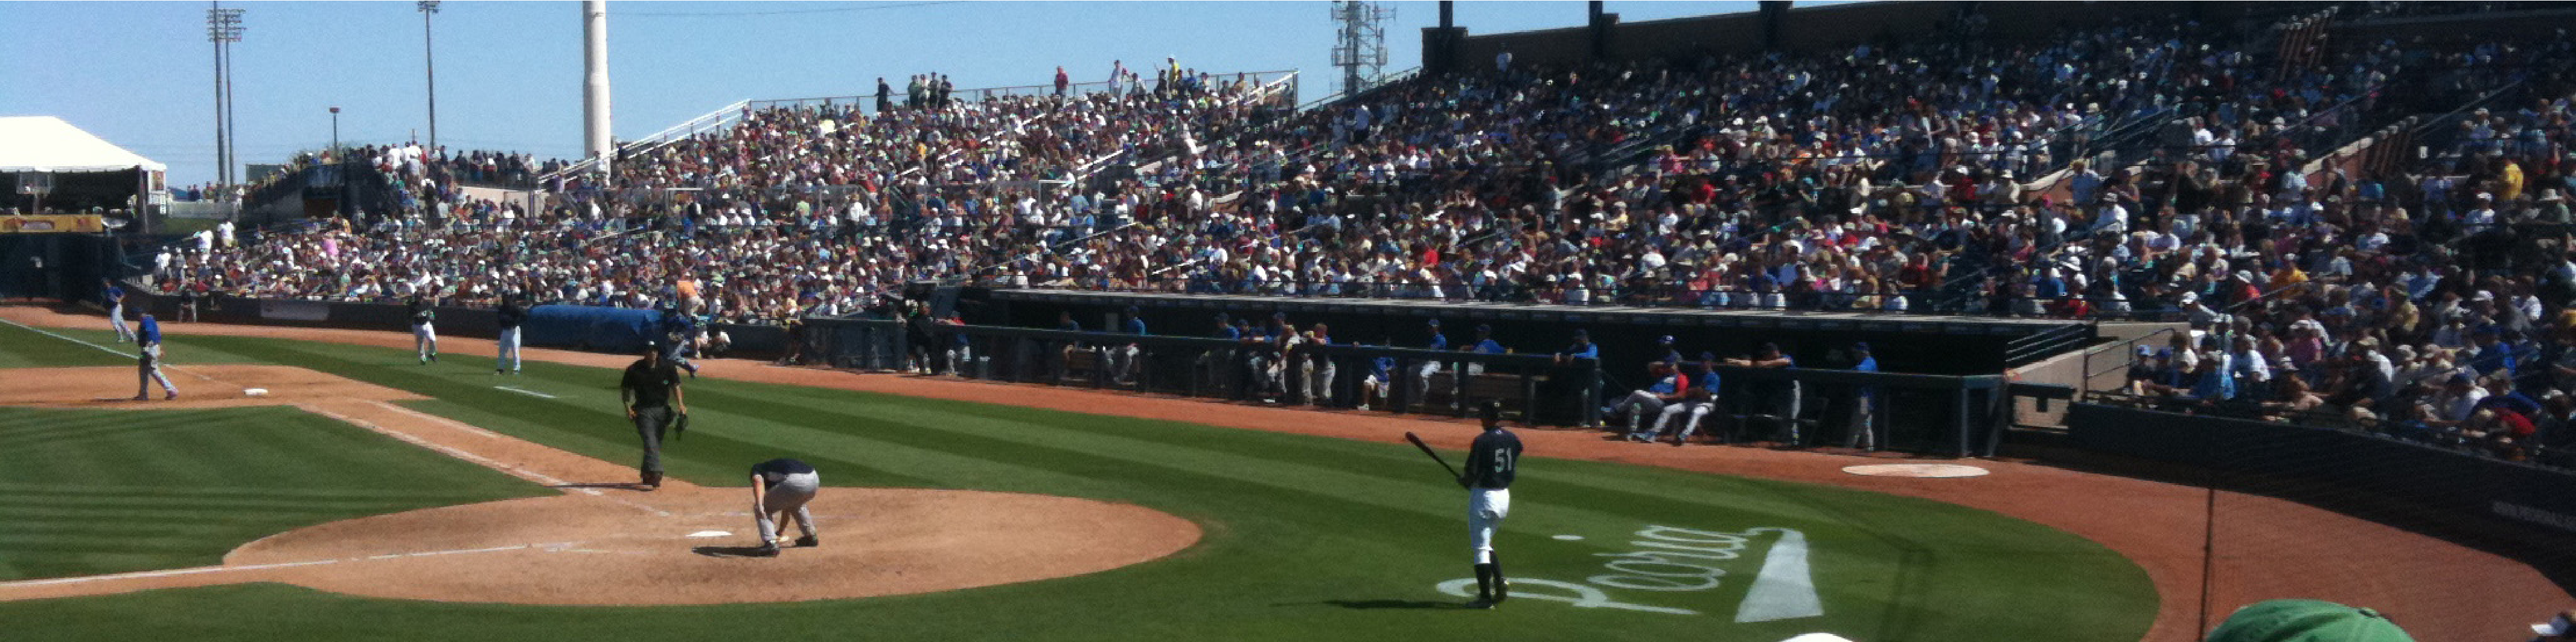
\includegraphics[width=\textwidth]{sampleteaser}
  \caption{This is a teaser}
  \label{fig:teaser}
\end{teaserfigure}


\maketitle

\hypertarget{introduction}{%
\section{Introduction}\label{introduction}}

``Tribute'' is the first single of Tenacious D's self-titled debut album\citep{Cowan1988, Whittaker2016-time-info}. It was released July 16, 2002. The song is a tribute to what Gass and Black refer to as ``The Greatest Song in the World'' (often confused as the song's title), which Tenacious D themselves came up with, but have since forgotten. It was released as a downloadable track for Rock Band in addition to appearing as a playable track for Guitar Hero Live.\citep{Hume1748}

\hypertarget{history}{%
\section{History}\label{history}}

Tribute was the first song Black and Gass played live as Tenacious D. The song, like many other songs that were recorded on Tenacious D, was originally performed on their short-lived HBO TV series. During earlier performances of this song Kyle Gass played the opening to ``Stairway to Heaven''. The two songs are both in A minor and have very similar chord progressions, and critics have said the songs sound alike.\citep{Cowan1988, Gluck2005, Wardak2002} \textbf{The maturation of the song over time is shown in Figure \ref{fig:tribute-plot}.}

\begin{figure}
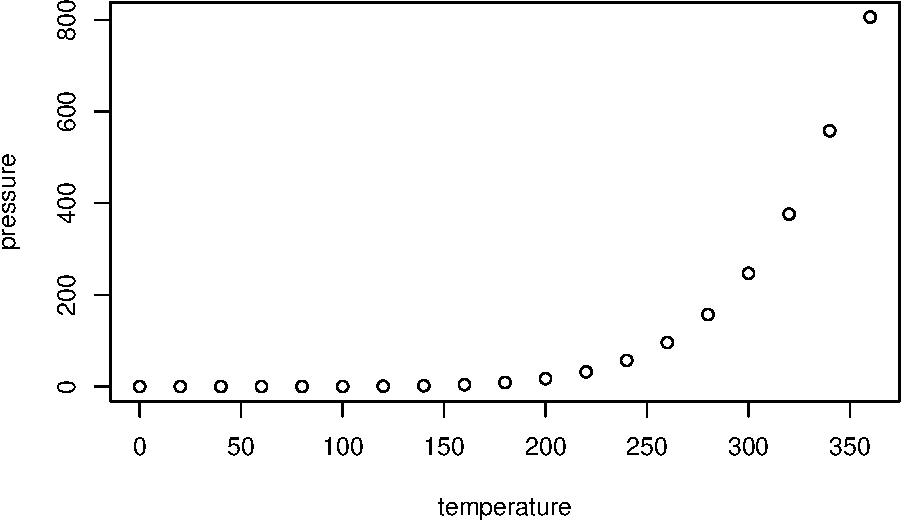
\includegraphics[width=0.98\columnwidth]{step6_files/figure-latex/tribute-plot-1} \caption{This is how great Tribute gets over time}\label{fig:tribute-plot}
\end{figure}

\begin{figure*}
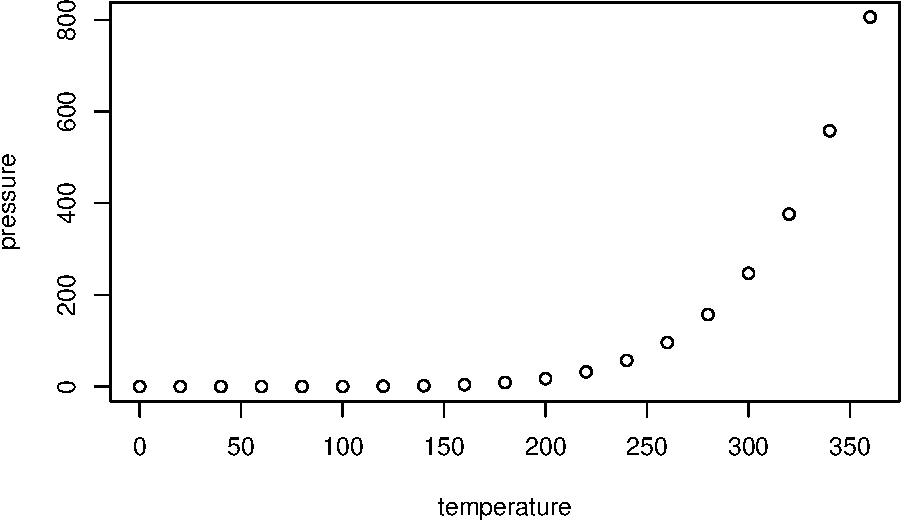
\includegraphics[width=0.98\textwidth]{step6_files/figure-latex/two-col-tribute-plot-1} \caption{This is a two-column plot of how great Tribute gets over time}\label{fig:two-col-tribute-plot}
\end{figure*}

\hypertarget{synopsis}{%
\subsection{Synopsis}\label{synopsis}}

The song chronicles the band members' encounter with a demon who demands the duo play ``the best song in the world'' or have their souls eaten. Having nothing to lose from trying, they play ``the first thing that came to our heads'', and it ``just so happened to be the best song in the world.''\citep{Wardak2002}

\begin{table}

\caption{\label{tab:table-iris}The favorite iris' of Tenacious D.}
\centering
\begin{tabular}[t]{rrrr}
\toprule
Sepal.Length & Sepal.Width & Petal.Length & Petal.Width\\
\midrule
5.1 & 3.5 & 1.4 & 0.2\\
4.9 & 3.0 & 1.4 & 0.2\\
4.7 & 3.2 & 1.3 & 0.2\\
4.6 & 3.1 & 1.5 & 0.2\\
5.0 & 3.6 & 1.4 & 0.2\\
\addlinespace
5.4 & 3.9 & 1.7 & 0.4\\
4.6 & 3.4 & 1.4 & 0.3\\
5.0 & 3.4 & 1.5 & 0.2\\
4.4 & 2.9 & 1.4 & 0.2\\
4.9 & 3.1 & 1.5 & 0.1\\
\bottomrule
\end{tabular}
\end{table}

Given the ``Stairway to Heaven'' interlude in the original TV series version, along with the similarity of the chord progression in both songs, Tribute at first implies that the best song in the world is indeed that song. However, the lyrics make clear that Tribute sounds nothing like the song they came up with to please the demon; as Black describes: ``And the peculiar thing is this my friends: The song we sang on that fateful night, it didn't actually sound anything like this song.''

\bibliographystyle{ACM-Reference-Format}
\bibliography{my-bibliography}

\end{document}
